\section{¿Por qué GIT?}
\usebackgroundtemplate{%
  
\includegraphics[width=\paperwidth,height=\paperheight]{imgs/git-no.jpg}} 
\frame
{
\frametitle{¿Por qué GIT?}
}

\usebackgroundtemplate{%
  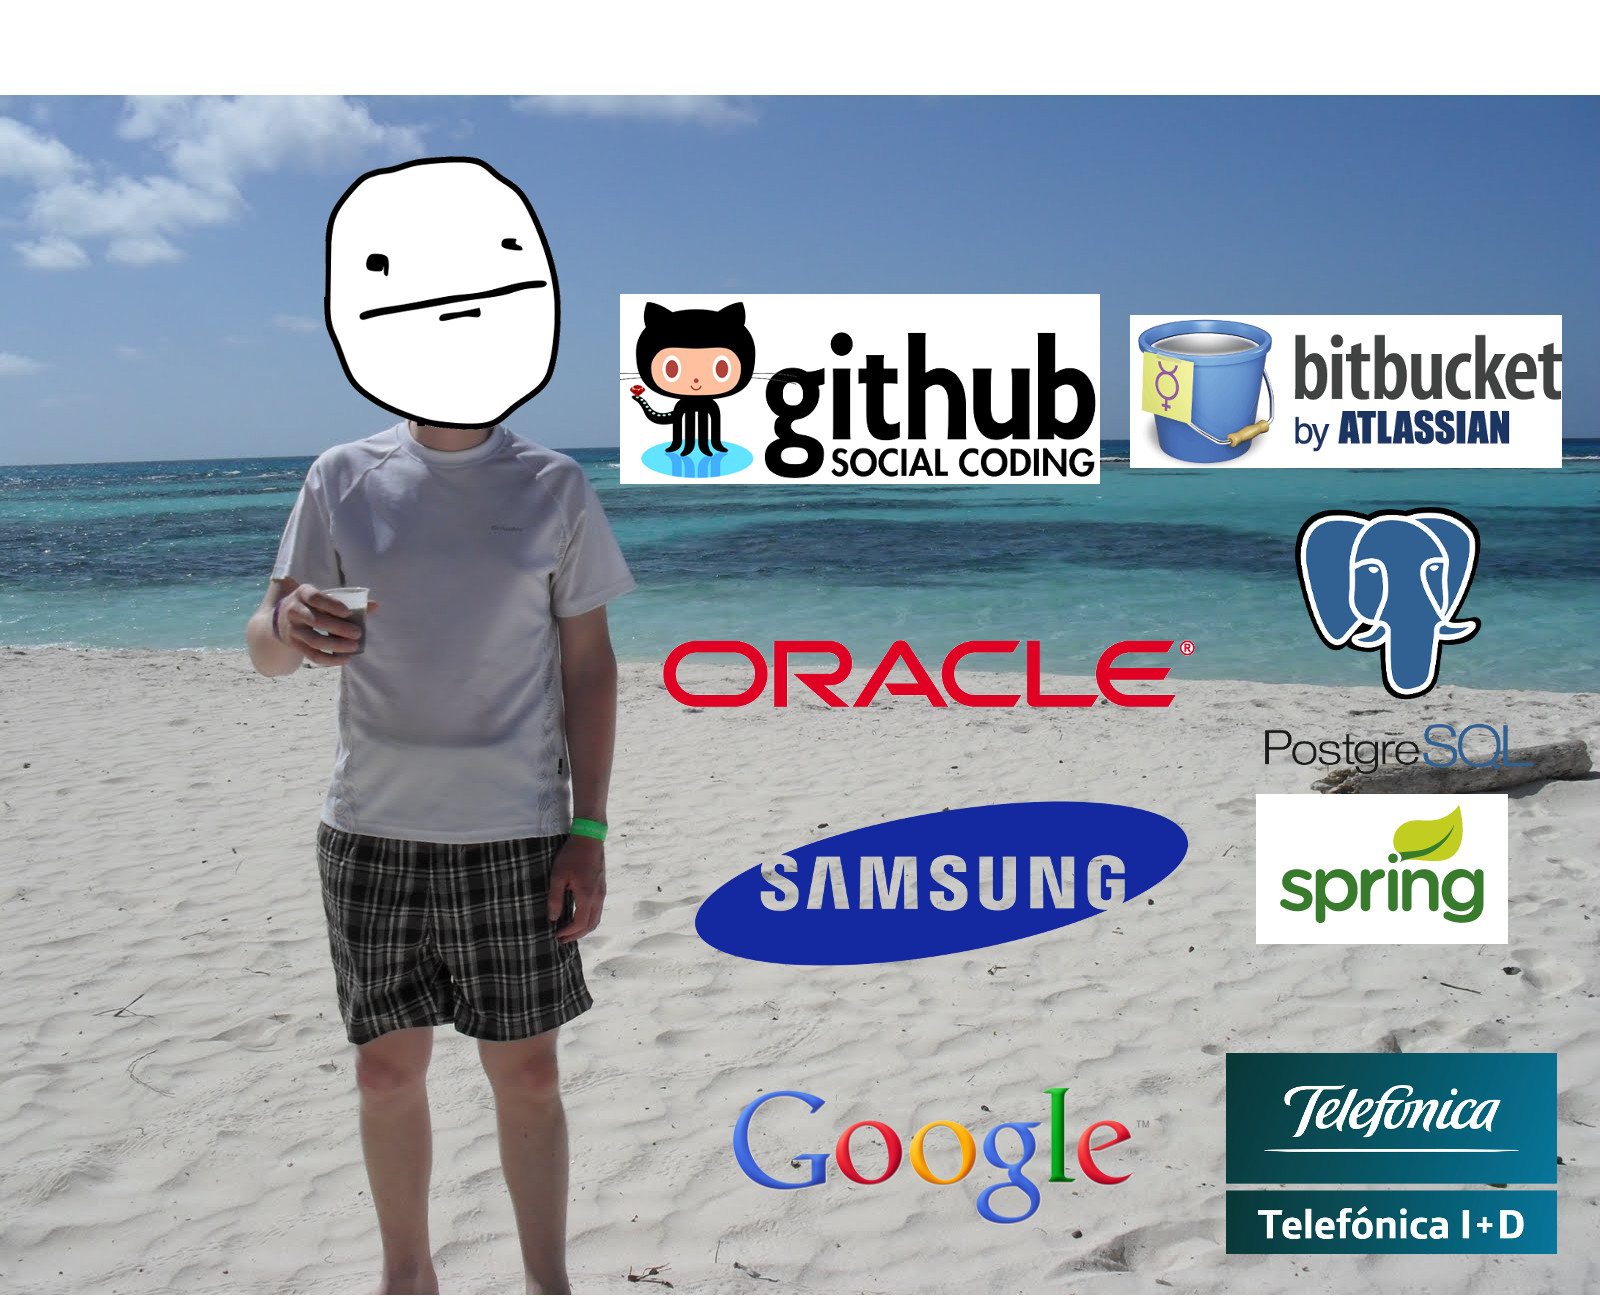
\includegraphics[width=\paperwidth,height=\paperheight]{imgs/git-si.jpg}} 
\frame
{
\frametitle{¿Por qué GIT?}
}
\usebackgroundtemplate{}
\frame
{
\frametitle{En números}

\includegraphics[height=1cm]{imgs/git-bitbucket.png}
\begin{itemize}
 \item Enfocado a \textbf{código privado} (Facebook, Cisco, Adobe, Opera...)
 \item Más de \textbf{1 millón} de usuarios registrados
 \item Integración del resto del ecosistema software: Bamboo (CI), Confluence (Doc), Jira (project tracking), SourceTree (GUI)...
 \item Se cobra por \textbf{número de integrantes de equipo}: 0-5 (gratis), 6-10 (\$10 month), 11-25 (\$25 month), 26-50 (\$50 month)...
\end{itemize}


\includegraphics[height=1cm]{imgs/git-github.png}
\begin{itemize}
 \item Enfocado a \textbf{código abierto} (bootstrap, nodejs, jquery...)
 \item Más de \textbf{4 millones} de usuarios registrados y \textbf{8 millones} de \textbf{repositorios} creados
 \item Se cobra por \textbf{repositorios privados}: 5 (\$7 month), 10 (\$12 month), 20 (\$22 month), 50 (\$50 month)
\end{itemize}
}
